% Build from output/pdf. Pages 2-4 retain the original PDF content; the sole
% architecture edit replaces the obsolete JSON-cache sentence on page 2.
\documentclass[11pt,a4paper]{article}
\usepackage[T1]{fontenc}
\usepackage[utf8]{inputenc}
\usepackage{lmodern,microtype}
\usepackage[margin=20mm,top=21mm,bottom=21mm,headheight=14pt]{geometry}
\usepackage{amsmath,amssymb,mathtools,booktabs,tabularx,array,longtable}
\usepackage{xcolor,enumitem,fancyhdr,titlesec,listings,pdfpages,hyperref,xurl,etoolbox}
\hypersetup{colorlinks=true,linkcolor=blue!45!black,citecolor=blue!45!black,urlcolor=blue!45!black,
 pdftitle={Mathematical Background and Implementation Guide for the N2 Index},
 pdfsubject={FORM, SQLite and sparse singlet projection for four-dimensional N=2 indices}}
\pagestyle{fancy}\fancyhf{}
\fancyhead[L]{\small\texttt{n2\_theory\_index.py}}
\fancyhead[R]{\small Mathematical background}
\fancyfoot[C]{\thepage}\renewcommand{\headrulewidth}{0pt}
\titleformat{\section}{\large\sffamily\bfseries}{\thesection}{0.6em}{}
\titleformat{\subsection}{\normalsize\sffamily\bfseries}{\thesubsection}{0.6em}{}
\setlength{\parindent}{0pt}\setlength{\parskip}{6pt}\setlength{\emergencystretch}{2em}
\setlist{itemsep=4pt,topsep=5pt,leftmargin=1.5em}
\renewcommand{\arraystretch}{1.18}
\newcolumntype{Y}{>{\raggedright\arraybackslash}X}
\newcommand{\code}[1]{{\small\nolinkurl{#1}}}
\BeforeBeginEnvironment{tabularx}{\par\noindent}
\AfterEndEnvironment{tabularx}{\par}
\newcommand{\PE}{\operatorname{PE}}
\newcommand{\adj}{\mathrm{adj}}
\lstset{basicstyle=\ttfamily\footnotesize,columns=fullflexible,keepspaces=true,
 breaklines=true,showstringspaces=false,backgroundcolor=\color{black!4},
 frame=single,rulecolor=\color{black!10},aboveskip=8pt,belowskip=8pt}
\begin{document}
\begin{center}
{\Large\sffamily\bfseries Mathematical Background and\\ Implementation Guide}\par
{\large\texttt{n2\_theory\_index.py}}\par
FORM and LiE computation of four-dimensional $\mathcal N=2$ indices\\
Simple and semisimple product gauge groups\par
\textbf{Index/cache revision: 10 September 2026}
\end{center}
\vspace{3mm}
\textbf{Purpose.} The canonical implementation computes the flavor-unrefined right
superconformal index of a Lagrangian four-dimensional $\mathcal N=2$ gauge theory.
FORM performs exact truncated series algebra. LiE decomposes individual Adams
operations and intermediate products. Python pairs dual irreps to extract the
final singlet, independently for every simple gauge factor. SQLite stores exact
parsed FORM expansions, decompositions and final singlet coefficients. Sage supplies input/representation
data, the dual-label convention and the exact returned polynomial ring.

This revision describes commit \code{04bbe21}: FORM expansion caching, reuse of
cached character factors, and a complete Adams-cache builder with a process pool.
It gives exact cutoff bounds, APIs and measured comparisons. The index convention
and single-letter equations are retained. Earlier validation is dated explicitly. The companion implementation reference provides package-wide context.

\section*{Contents}
\begin{tabularx}{\textwidth}{@{}Yr@{}}
1 Scope and program architecture & 2\\
2 Index convention and single-letter functions & 2\\
3 Matter characters for simple and product groups & 3\\
4 Plethystic exponential and exact cutoffs & 3\\
5 How FORM represents and expands the index & 3\\
6 Adams operations and LiE decomposition & \pageref{sec:adams}\\
7 Gauge-singlet projection for product groups & \pageref{sec:projection}\\
8 SQLite caches and complete Adams-cache builder & \pageref{sec:cache}\\
9 Python functions and their mathematical roles & \pageref{sec:functions}\\
10 JSON examples and command-line use & \pageref{sec:json}\\
11 Validation and representative performance & \pageref{sec:validation}\\
12 Interpretation and limitations & \pageref{sec:limits}\\
References & \pageref{sec:refs}\\
\end{tabularx}
\clearpage
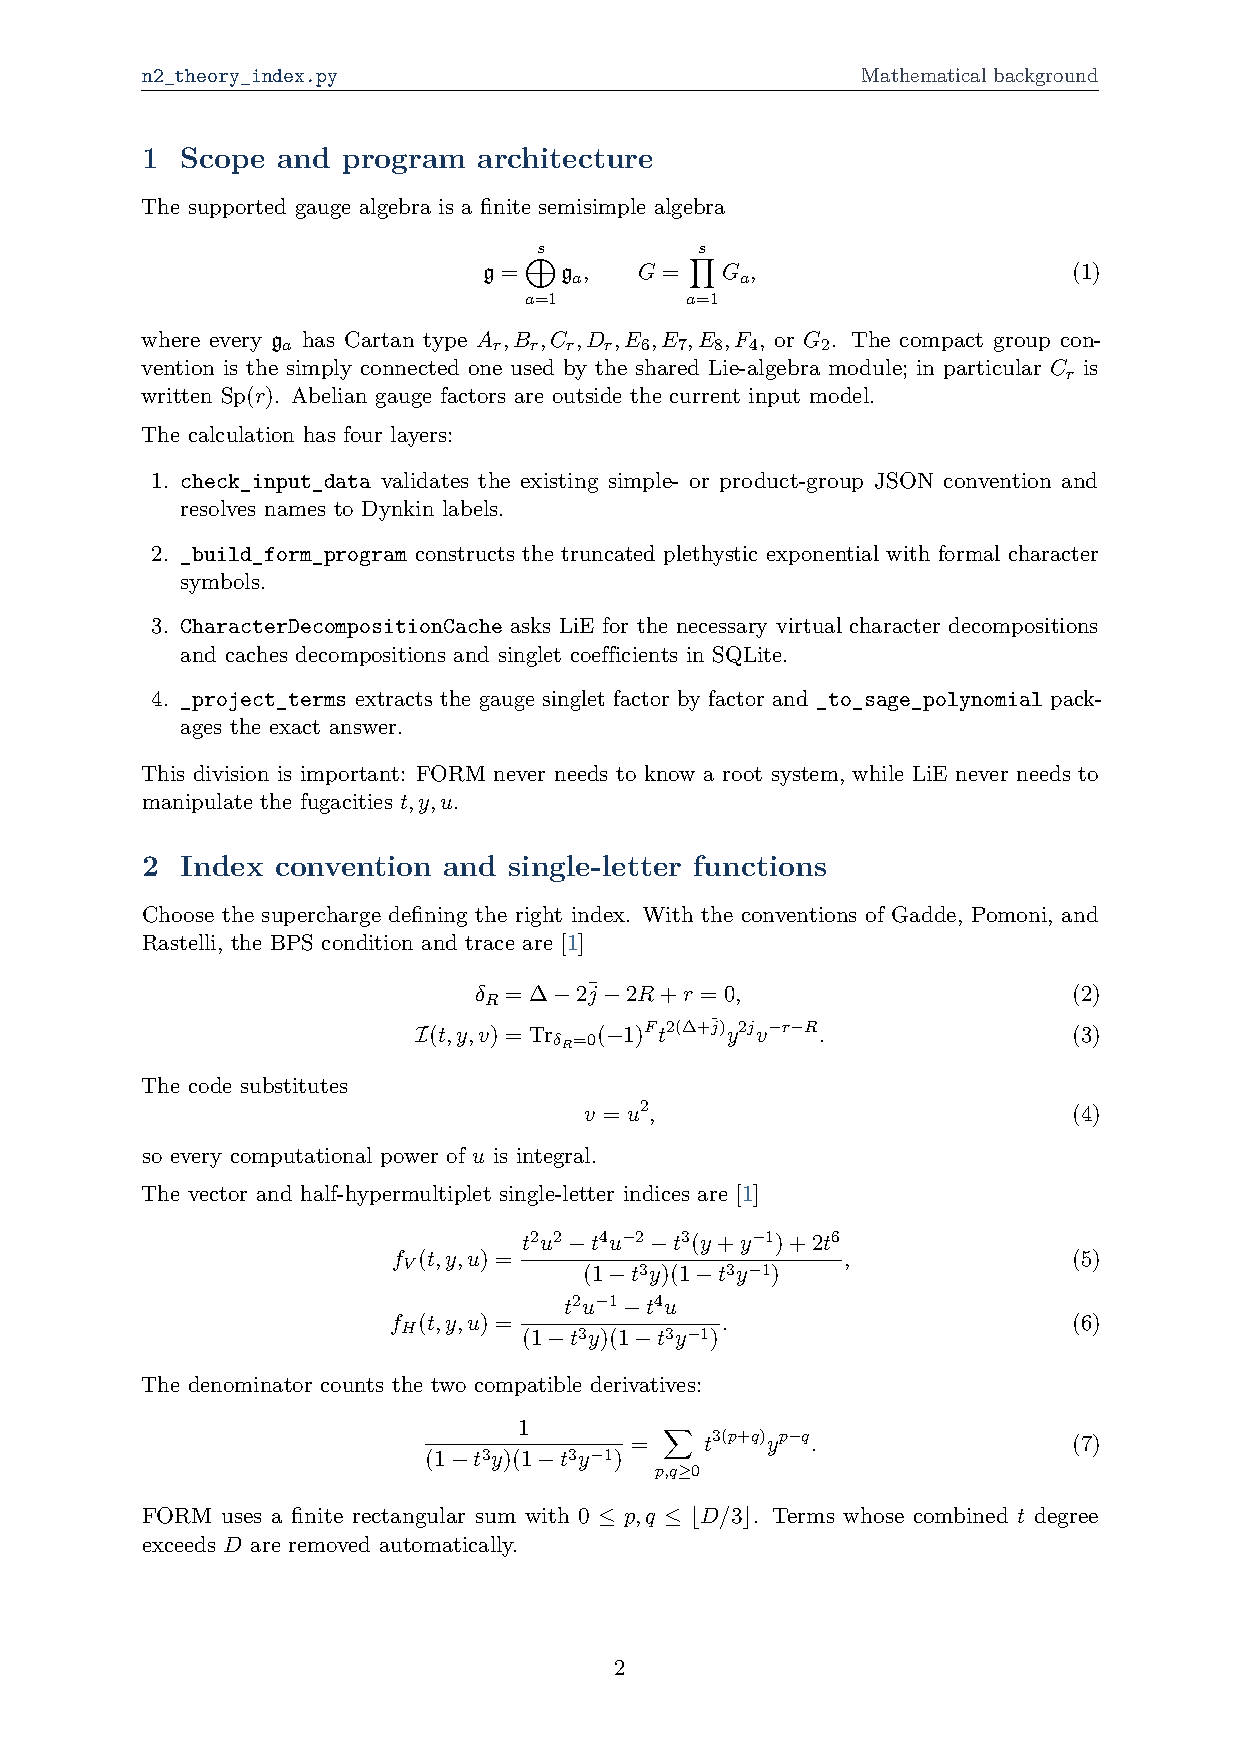
\includepdf[pages=-,pagecommand={\thispagestyle{empty}}]{source_assets/n2_background_preserved_pages_2_to_4.pdf}
\setcounter{section}{5}\setcounter{subsection}{3}\setcounter{equation}{18}
After the $k$-th step, induction gives
\begin{equation}
 I_k=\sum_{r=1}^{k-1}\frac{E^r}{r!}+z\frac{E^k}{k!}.
\end{equation}
The final substitution $z\mapsto1$, followed by adding the vacuum term, yields
\begin{equation}
 1+I_M=\sum_{r=0}^{M}\frac{E^r}{r!}=\exp(E)+O(t^{D+1}).
\end{equation}
This is an ordinary exponential of a representation-valued series; Bose and Fermi
statistics have already entered through the signed single-letter functions.

\section{Adams operations and LiE decomposition}\label{sec:adams}
\subsection{The representation-ring calculation}
For each irrep $R$ and exponent vector $\mathbf n=(n_1,n_2,\ldots)$, the cache
stores the virtual decomposition
\begin{equation}
 D_R(\mathbf n)=\operatorname{Decomp}\left[\bigotimes_{j\geq1}
 (\psi^jR)^{\otimes n_j}\right].
\end{equation}
An Adams operation scales every weight by $j$ and can produce a virtual
representation with negative coefficients \cite[Secs.~3.4, 4.5]{lie}. For the
$A_1$ fundamental,
\begin{equation}
 \psi^2(\mathbf2)=\mathbf3-\mathbf1,
\end{equation}
which LiE prints as a signed decomposition polynomial.

\subsection{The LiE commands in plain language}
\begin{tabularx}{\textwidth}{@{}p{57mm}Y@{}}
\toprule LiE expression & Meaning\\\midrule
\code{Adams(2,[1],A1)} & Decomposes $\psi^2$ of the $A_1$ irrep with label
$[1]$; the result is \code{-1X[0]+1X[2]} \cite[Sec.~4.5]{lie}.\\
\code{tensor([1],[1],A1)} & Returns \code{1X[0]+1X[2]} for
$V_{[1]}\otimes V_{[1]}$ \cite[Sec.~4.5]{lie}.\\
\code{tensor(p,q,A1)} & Tensors two decomposition polynomials. The revised
projector uses this for intermediate products only.\\
\code{tensor(p,q,[0],A1)} & LiE's targeted trivial coefficient operation.
The revised projector instead performs the final dual-irrep pairing in Python.\\
\code{maxnodes N / maxobjects N} & Raises LiE node/object limits. The code
retries with these settings only after a failed ordinary run, avoiding eager
large-allocation startup cost \cite[Sec.~2.3]{lie}.\\\bottomrule
\end{tabularx}
A decomposition polynomial has the form
\begin{equation}
 p=\sum_{\lambda\in P_+}m_\lambda X[\lambda_1,\ldots,\lambda_r],\qquad m_\lambda\in\mathbb Z.
\end{equation}
The parser preserves the signed integer $m_\lambda$. It also removes LiE's
optional ``New tree space with maximum number of nodes'' notification by
recognizing the message prefix, rather than by deleting a fixed number of output characters.

\clearpage
\section{Gauge-singlet projection for product groups}\label{sec:projection}
The gauge index is the Haar projection
\begin{equation}
 \mathcal I(t,y,u)=\int_G d\mu_G(g)\,Z(t,y,u;g).
\end{equation}
Equivalently, it is the multiplicity of the trivial representation in every coefficient.
After FORM expansion, a typical formal-character monomial is
\begin{equation}
 \mathcal C=\prod_p\prod_{j\geq1}C_p(j)^{n_{p,j}}.
\end{equation}
If $a(p)$ is the gauge factor associated with character $p$, define the virtual
$G_a$ representation
\begin{equation}
 X_a(\mathcal C)=\bigotimes_{p:\,a(p)=a}\bigotimes_{j\geq1}(\psi^jR_p)^{\otimes n_{p,j}}.
\end{equation}
Because both the group and normalized Haar measure factorize,
\begin{align}
 d\mu_G&=\prod_{a=1}^s d\mu_{G_a},\\
 \operatorname{mult}_{\mathbf1_G}(\mathcal C)&=
 \prod_{a=1}^s\operatorname{mult}_{\mathbf1_a}\bigl(X_a(\mathcal C)\bigr).
\end{align}
This is the precise rule implemented by \code{_project_terms}. It partitions a
FORM term by gauge-factor position, batches distinct character-product singlet
requests for each factor, and multiplies the returned integers. Empty character
products have singlet multiplicity one. SQLite is checked before decomposition.

\subsection{Exact pairing from character orthogonality}
For compact $G$ and normalized Haar measure,
\begin{equation*}
 \int_G\chi_\lambda(g)\overline{\chi_\mu(g)}\,d\mu(g)=\delta_{\lambda\mu},
 \qquad \chi_{\mu^*}=\overline{\chi_\mu}.
 \tag{28a}
\end{equation*}
Thus for two partial virtual characters,
\begin{equation*}
 A=\sum_\lambda a_\lambda\chi_\lambda,\quad
 B=\sum_\mu b_\mu\chi_\mu,\qquad
 \boxed{[\mathbf1](AB)=\sum_\lambda a_\lambda b_{\lambda^*}.}
 \tag{28b}
\end{equation*}
Character orthogonality is Corollary 35.9 of \cite{etingof}. Equation (28b) follows
by substitution and linearity, including negative coefficients. Equivalently,
$(V\otimes W)^G\simeq\operatorname{Hom}_G(V^*,W)$; the latter is the space of
linear maps commuting with the group action. Schur's lemma selects dual irreps.
The singlet functional here is bilinear; an ordinary coefficient dot product
would incorrectly pair complex irreps with themselves.

\clearpage
\subsection{Split before decomposition}
A symbolic input \code{(labels, (n1,n2,...))} stands for
$\prod_j\psi^j(R)^{n_j}$. The revised procedure is:
\begin{enumerate}
\item Remove trivial-character factors, since $\psi^j(\mathbf1)=\mathbf1$.
\item Expand exponents into individual Adams factors and split them into two
approximately balanced parts $A$ and $B$.
\item Fully decompose the needed \emph{partial} products, reusing persistent and
in-memory entries. Individual Adams operations remain indivisible.
\item Apply (28b) using sparse dictionary lookups and save the resulting integer.
\end{enumerate}
The splitter's cost estimate for an atom is
\begin{equation*}
 c(\lambda,j)=j\max\left(1,\sum_i\lambda_i\right).
 \tag{28c}
\end{equation*}
It places larger estimates first on the currently lighter side, preferring an
already-present base irrep when the two costs tie. This source-derived heuristic
balances approximate highest-weight sizes, not exact tensor complexity, and
carries no optimality guarantee. Repeated factors of one base irrep can be split
across the two sides before their complete product is decomposed.

For example, $\psi^4(\adj)\psi^5(\adj)$ needs only the two individual Adams
expansions and their pairing. In contrast, $\psi^3(\adj)^3$ leaves the intermediate
$\psi^3(\adj)^2$, which can remain expensive. The full decomposition API is still
available when explicitly requested; the singlet path avoids tensor-decomposing
the complete product.

\subsection{Dual labels and signed examples}
The highest weight of the dual irrep is
\begin{equation*}
 \lambda^*=-w_0\lambda.\tag{28d}
\end{equation*}
The map permutes fundamental weights \cite[Prop.~32.1]{etingof}.
\code{_dual_permutation} obtains that permutation with the existing Sage duality
helper and caches it; \code{_singlet_pair} applies it to label tuples.
See also Sage's \code{dual()} and \code{inner_product()} \cite{sage}.
The pairing iterates over the smaller support, using $O(r\min(N_A,N_B))$ label
operations. The costly step can still be constructing $A$ or $B$.

For $SU(3)$, $(a,b)^*=(b,a)$, so
$[\mathbf1](\mathbf3\otimes\overline{\mathbf3})=1$ but
$[\mathbf1](\mathbf3\otimes\mathbf3)=0$. Actual conjugate orientations must remain
in cache keys, even where theory enumeration identifies conjugates.
For $SU(2)$, $\mathbf2\otimes\mathbf2=\mathbf1\oplus\mathbf3$ implies
$[\mathbf1](\mathbf2^{\otimes4})=1^2+1^2=2$. Pseudoreality adds no sign to this
pairing. Signed Adams coefficients are different: from (22),
$[\mathbf1](\psi^2\mathbf2)=-1$, while
$[\mathbf1]((\psi^2\mathbf2)^2)=(-1)^2+1^2=2$.

\clearpage
\section{SQLite caches and complete Adams-cache builder}\label{sec:cache}
For the exponent vector in Eq.~(21), define its total Adams order
\begin{equation}
 q(\mathbf n)=\sum_{j\geq1}j n_j.
\end{equation}
The default local file is \code{<project-root>/char_decomposition_cache.db}.
Python's \code{sqlite3} stores both full character decompositions and final
singlet integers. The schema has \code{user_version=1}, independently of the
MySQL theory database. There is no combined product-group decomposition table;
identical simple factors reuse the same entries.

\begin{tabularx}{\textwidth}{@{}p{50mm}Y@{}}
\toprule Table & Columns and primary key\\\midrule
\code{character_decompositions} & \code{algebra} \code{TEXT}, \code{dynkin_labels} \code{TEXT},
\code{adams_powers} \code{TEXT}, \code{adams_order} \code{INTEGER}, \code{terms_json} \code{TEXT}.
Key: \code{(algebra, dynkin_labels, adams_powers)}.\\[4pt]
\code{singlet_coefficients} & \code{algebra} \code{TEXT}, \code{product_key} \code{TEXT},
\code{coefficient} \code{TEXT}. Key: \code{(algebra, product_key)}.\\\bottomrule
\end{tabularx}
All columns are non-null, and both tables use \code{WITHOUT} \code{ROWID}. Label and
power tuples are compact JSON text; signed coefficients are decimal strings,
avoiding SQLite's 64-bit integer limit \cite{sqlite-types}. Decomposition payloads
are lists of \code{[labels, "coefficient"]} pairs. The full power tuple is required:
total Adams order alone does not distinguish, for example, $R^{\otimes2}$ from
$\psi^2(R)$.

Symbolic singlet keys contain \code{["characters", canonical_product]}.
Repeated base labels merge by adding exponents; factors sort in descending order.
Already-decomposed inputs use a separate \code{"decompositions"} namespace.
Zeros and negative coefficients are valid cache hits. Returned decompositions
are copies, so caller mutation does not change a cached entry.

\subsection{Lookup order and concurrency}
A singlet lookup checks thread-local memory, then SQLite, before requesting any
partial decomposition. Same-base-irrep partial products use persistent entries;
mixed partial decompositions live only in the thread-local \code{partial_products}
dictionary. Only the final complete-product scalar is persisted as a singlet.

Each thread owns a connection. PID checks avoid inherited connections; before
starting a process pool the parent closes its connection. Workers calculate
independent requests, and the parent batches completed writes by dependency
level. Sequential batches flush after 64 entries and at completion. LiE work
occurs outside write transactions. Failed calculations do not cache a guessed zero.

WAL allows concurrent readers and a writer, while writers remain serialized;
it assumes a local filesystem \cite{sqlite-wal}. The code uses a 30-second busy
timeout and bounded retries. Python connection contexts manage transactions;
this cache's context manager additionally closes the connection and clears
thread-local entries \cite{python-sqlite}.

Legacy JSON file discovery/import and \code{cache_path()} are removed. The new
projection preserves existing SQLite keys and schema; no migration is needed.
FORM expansion now has its own raw-program cache, described next.
\newcommand{\cacheheading}{\subsection}
% Shared by the two standalone PDF documents. The caller defines \cacheheading.
% New displays are unnumbered to preserve the existing equation numbering.
\clearpage
\cacheheading{Persisting the FORM expansion before projection}
\code{index/form_expansion_cache.py} now owns \code{IndexFormTerm}, the exact
parser, and \code{FormExpansionCache}. For raw program text $P$, the stored value is
the parsed list of monomials before any gauge projection:
\[
 P\longmapsto \left\{\left(c,\alpha,\beta,\gamma,
        ((p,\mathbf n_p))_p\right)\right\},\qquad
 c\,t^\alpha y^\beta u^\gamma\prod_{p,j}C_p(j)^{n_{p,j}}.
\]
This notation is a direct description of the project record format. Each
\code{IndexFormTerm} has a \code{Fraction} coefficient, integer fugacity powers,
and a tuple of character indices and Adams-power tuples. The compact JSON row is
\code{["numerator", "denominator", t_power, y_power, u_power, characters]}.
\code{_encode_expansion} stores a list of these rows; \code{_decode_expansion}
restores exact arbitrary-size fractions and nested tuples. No float conversion
or representation decomposition occurs in this layer.

\begin{lstlisting}[language=SQL]
CREATE TABLE form_expansions (
    program TEXT COLLATE BINARY NOT NULL PRIMARY KEY,
    expansion_json TEXT NOT NULL
) WITHOUT ROWID;
\end{lstlisting}
The key is the complete program text, compared verbatim, not a hash. Whitespace,
numeric multiplicities, symbol names and the truncation order matter. There is
no program normalization or symbolic-multiplicity template. The default file is
\code{form_expansion_cache.db}, separate from the character database; the FORM
module does not set a separate \code{user_version}.

\textbf{Lookup.} \code{get_expansion(program)} reads and decodes a hit. A miss
runs \code{run_form}, calls \code{parse_form_output}, encodes the terms and
commits with \code{ON CONFLICT (program) DO NOTHING}. Failed execution or parsing
does not create an entry. Each thread opens its own connection, with a PID check
before reusing it, WAL, a 30-second busy timeout and up to three attempts for
busy/locked writes. FORM runs outside write transactions. Concurrent identical
misses can execute FORM more than once, but retain only one complete row.
The context manager closes the current thread's connection. These boundaries
follow the implementation and SQLite's serialized-writer model \cite{sqlite-wal,python-sqlite}.

\textbf{Index integration.} \code{calculate_index} and
\code{calculate_index_internal} accept \code{form_cache_database_path=}; the
index CLI exposes \code{--form-cache-database}. Otherwise the FORM database is
placed beside the selected character database. A hit bypasses FORM execution
and FORM-output parsing, while group-specific singlet projection still runs.
Orders below two return the vacuum without external execution or cache access.

Different theories can share this expansion when their raw programs are
identical and they use the same FORM database. Group and irrep meanings are
supplied afterward by each theory's character basis. Their final indices can
therefore differ despite a shared expansion. This reuse applies to the supported
non-$SU$ groups too; it does not require a power-sum/Schur integration backend.

\clearpage
\cacheheading{Reusing lower-order character decompositions}
Write the cached virtual character as
\[
 D_R(\mathbf n)=\sum_\lambda d_\lambda\chi_\lambda
   =\prod_{j\geq1}(\psi^j\chi_R)^{n_j},\qquad
 q(\mathbf n)=\sum_j j n_j.
\]
If $\mathbf a+\mathbf b=\mathbf n$ componentwise, multiplication in the
representation ring gives
\[
 D_R(\mathbf n)=D_R(\mathbf a)D_R(\mathbf b),\qquad
 d_\nu=\sum_{\lambda,\mu}
     a_\lambda b_\mu N_{\lambda\mu}^{\nu},
 \quad \chi_\lambda\chi_\mu=\sum_\nu N_{\lambda\mu}^{\nu}\chi_\nu.
\]
The identity follows by multiplying the defining Adams products; LiE's
\code{tensor} implements the last decomposition \cite[Sec.~4.5]{lie}.
Signed coefficients remain valid. The two exact base cases are
$D_R(\mathbf e_1)=\chi_R$ and $D_{\mathbf1}(\mathbf n)=1$;
neither needs a LiE call.

\code{CharacterDecompositionCache._decomposition_dependencies} first tries the
usual split: remove one factor at the smallest occupied Adams index. For at most
two factors, or when both usual dependencies are available, it retains that
split. Otherwise it searches lower-weighted-order keys for the \emph{same}
Cartan type and Dynkin labels, including thread-local entries and the known
first Adams operation. It considers pairs already available whose padded
exponent vectors sum to the requested vector.

Among alternative pairs, the score is the product of the two numbers of
irreducible terms, with zero cost for a zero or scalar-trivial factor. Ties use
the total number of terms and then the vectors themselves. This estimates
tensor work; it does not predict the fastest LiE call or find a globally optimal
factorization. The batch dependency planner and the actual calculation use the
same selection. Existing SQLite keys, schema and thread/process ownership are
unchanged.

For example, if $R^{\otimes2}$ and $(\psi^2R)^{\otimes2}$ are stored, their
product can be obtained with one tensor operation on those entries. Atomic
prerequisites need not be recalculated just to reconstruct a cached composite.
On-demand generation still constructs missing prerequisites when no suitable
cached split is available. It does not automatically enumerate all lower orders.

\textbf{Scope.} This optimization is separate from the singlet splitter. The
singlet path still decomposes two partial products and contracts dual labels;
the new dependency choice helps construct the required same-irrep partial
products. Intermediate full tensor decompositions can remain expensive even
when all individual Adams operations have already been cached.

\clearpage
\cacheheading{Building every product through a chosen Adams order}
\code{build_decomposition_cache(cartan_type, dynkin_labels, max_adams_order, ...)}
in \code{index/char_decomposition_cache.py} fills the existing decomposition
table for one base irrep. At weighted order $q$ it calls
\code{common.math_utils.frobenius_solve(range(1, q + 1), q)} to enumerate
\[
 \mathcal P_q=\left\{(n_1,\ldots,n_q)\in\mathbb Z_{\geq0}^q:
                 \sum_{j=1}^{q}j n_j=q\right\}.
\]
Each solution specifies one Adams product. This is also the multiplicity
description of an integer partition: $|\mathcal P_q|=p(q)$, with counts
$1,2,3,5,7,11$ at orders one through six (29 rows in total).

Orders run sequentially. The builder reads existing keys at the current order,
skips complete rows without decoding their payloads, and divides missing
solutions into batches for a persistent \code{ProcessPoolExecutor} using
\code{spawn}. Batches contain at most 64 requests, with several batches per
worker to balance uneven costs. Workers read prerequisites and calculate;
the parent commits each returned batch. It submits the next order only after
the current one is fully committed. LiE never runs in a write transaction.
Completed batches survive a later failure or interruption, so a rerun resumes
from the missing entries. Independent builders may duplicate simultaneous
misses; uniqueness and short transactions preserve complete stored rows.

Every composite at order $q$ has a split into two strictly lower orders.
Consequently both factors are already stored and at most one tensor operation
is needed for that request, with scalar/zero shortcuts as usual. For an initially
empty cache of a nontrivial irrep, one uninterrupted build needs only one
individual Adams calculation per $j=2,\ldots,M$: $M-1$ in total. This counts
logical Adams calculations, not backend retries or concurrent duplicate builds.
The builder fills same-irrep decompositions, not singlet coefficients, mixed-irrep
products or the FORM database.

\textbf{Cutoff for the full index.} A letter starts at $t^2$, and its $j$-th
Adams contribution starts no earlier than $t^{2j}$. For each base irrep in a
fixed gauge factor, its product therefore satisfies
\[
 \deg_t\ \geq\ 2\sum_j j n_j=2q
 \quad\Longrightarrow\quad
 q\leq\left\lfloor\frac{N}{2}\right\rfloor
 \quad\hbox{for an index through }t^N.
\]
This is a bound derived from the implemented single-letter functions. Use
$M=\lfloor N/2\rfloor$ for each required adjoint and matter irrep, retaining
distinct conjugate labels. It is a sufficient bound, not a claim that every
partition will occur in the projector. For product groups it holds factorwise;
one bifundamental letter contributes a character to multiple factors, so one
must not sum their separate orders and apply the same bound to that sum.
Through $t^{18}$, $M=9$ suffices. For $N<2$ there is no cache to prebuild.

\clearpage
\cacheheading{Builder API, dependencies and command-line examples}
With Sage's environment active, prepare the $A_2$ fundamental through order nine:
\begin{lstlisting}[language=bash]
sage -python -m index.char_decomposition_cache A2 \
  --dynkin-labels 1 0 --max-adams-order 9 --processes 4 \
  --cache-database /tmp/index-demo/char_decomposition_cache.db
\end{lstlisting}
Repeat for every required irrep. For $A_2$ SQCD these include $(0,1)$ and the
adjoint $(1,1)$ in addition to $(1,0)$. The group rank does not multiply the
maximum Adams order. The direct script entry point
\code{sage -python index/char_decomposition_cache.py ...} is also supported.

\begin{lstlisting}[language=Python]
from index.char_decomposition_cache import build_decomposition_cache

if __name__ == "__main__":
    totals = build_decomposition_cache(
        "A2", (1, 0), 9, processes=4,
        database_path="/tmp/index-demo/char_decomposition_cache.db",
        progress=lambda q, total, computed:
            print(q, total, computed),
    )
\end{lstlisting}
The return value is \code{dict[int, int]} mapping each order to its total product count, including reused
rows. The optional callback receives \code{(order, total, computed)} in the
parent after that order is committed. \code{processes=1} is serial; the default
is the available CPU count. The pool starts only when there is parallel work.
Use a \code{__main__} guard in scripts with multiple processes.

The maximum order and worker count must be positive integers. Cartan type,
rank and Dynkin labels are validated. \code{cache_directory=} and
\code{database_path=} are mutually exclusive. Other keywords are
\code{lie_executable=} and \code{timeout=} (600 seconds per LiE call by default;
Python accepts \code{None} for no timeout). The CLI provides
\code{--max-order} as an alias for \code{--max-adams-order}, as well as
\code{--cache-directory}, \code{--lie-executable}, and numeric \code{--timeout}.
It prints computed/reused counts and exits with status 2 on a reported failure.

The builder imports \code{frobenius_solve} lazily and therefore needs OR-Tools
only when called; ordinary index/cache lookups do not acquire that dependency.
Its enumeration and complete decompositions can grow much faster than the subset
used by one index. Prebuilding is optional, and a fully warm repeat still
enumerates solutions and checks keys even though it runs no LiE or worker pool.

Use the prepared character database and a shared FORM database for index calls:
\begin{lstlisting}[language=bash]
sage -python -m index.n2_theory_index theory.json --order 18 \
  --cache-database /tmp/index-demo/char_decomposition_cache.db \
  --form-cache-database /tmp/index-demo/form_expansion_cache.db
\end{lstlisting}
Without the last option, the FORM database defaults to that same directory.
The corresponding index Python keyword is \code{form_cache_database_path=}.


\clearpage
\section{Python functions and their mathematical roles}\label{sec:functions}
\begin{tabularx}{\textwidth}{@{}p{65mm}Y@{}}
\toprule Function or class & Mathematical/computational role\\\midrule
\code{_parse_input} & Resolves the ordered factors in Eq.~(1) and validated hypermultiplet data.\\
\code{_matter_character_multiplicities} & Constructs Eq.~(10), omits trivial factor
characters, and applies conjugation as in Eq.~(11).\\
\code{_character_basis} & Assigns each pair $(a,R)$ one FORM function $C_p$ and
records vector and matter character monomials.\\
\code{_build_form_program} & Implements Eqs.~(7), (17), (14), and (20).\\
\code{run_form} & Shared helper in \code{common/form_utils.py}; runs FORM in an
isolated temporary directory and requires a successful, clean process result.\\
\code{FormExpansionCache.}\newline\code{get_expansion} & Retrieves parsed terms by raw program;
executes, parses and stores a miss.\\
\code{FormExpansionCache.}\newline\code{parse_form_output} & Converts exact FORM monomials to
\code{IndexFormTerm} records with \code{Fraction} coefficients.\\
\code{get_decomposition},\newline\code{get_decompositions} & Retrieve or construct
Eq.~(21); prefer available cached factors and batch missing prerequisites by
tensor-factor count.\\
\code{build_decomposition_cache} & Enumerate all products at each weighted order;
commit lower orders before parallel generation of the next.\\
\code{get_singlet_multiplicities} & Look up symbolic-product singlets first;
calculate missing integers with \code{_character_singlets}.\\
\code{singlet_multiplicities} & Cache singlets from already-decomposed inputs;
misses call \code{_compute_singlet_multiplicities}.\\
\code{_split_character_product} & Greedily split individual Adams factors using
Eq.~(28c). Repeated factors may separate.\\
\code{_character_singlets} & Internal \code{plan()} identifies needed parts;
\code{expand()} builds and memoizes mixed parts before final pairing.\\
\code{_dual_permutation},\newline\code{_singlet_pair} & Cache the label permutation
in Eq.~(28d) and evaluate Eq.~(28b), including signed coefficients.\\
\code{_tensor_decompositions} & LiE decomposition of intermediate products;
zero and scalar-trivial factors are handled directly.\\
\code{_compute_singlet_multiplicities} & For decomposed inputs, sort by support
size, recursively build two parts and pair dual labels.\\
\code{_project_terms} & Multiplies factorwise singlet multiplicities and collects
equal powers of $t,y,u$.\\
\code{_to_sage_polynomial} & Returns an exact flat Laurent polynomial in
$\mathbb Q[t^{\pm1},y^{\pm1},u^{\pm1}]$; performs no representation calculation.\\
\code{calculate_index} & Coordinates the complete public in-memory calculation.\\
\code{calculate_index_from_file} & Loads JSON and delegates to \code{calculate_index}.\\\bottomrule
\end{tabularx}

\clearpage
\section{JSON examples and command-line use}\label{sec:json}
A simple-factor theory retains the existing form:
\begin{lstlisting}
{
    "algebra": "A2",
    "hypermultiplets": [
      {"representation": "fundamental", "number": 6, "kind": "full"}
    ]
}
\end{lstlisting}
A product theory names every gauge factor. Missing entries in
\code{representations} mean singlets:
\begin{lstlisting}
{
    "gauge_groups": [
       {"id": "left", "algebra": "A1"},
       {"id": "right", "algebra": "A1"}
    ],
    "hypermultiplets": [{
       "representations": {
          "left": "fundamental", "right": "fundamental"
       },
       "number": 2, "kind": "full"
    }]
}
\end{lstlisting}
With the Sage environment active and \code{form} and \code{lie} on \code{PATH}:
\begin{lstlisting}[language=bash]
python -m index.n2_theory_index theory.json --order 10
\end{lstlisting}
The default files are \code{char_decomposition_cache.db} and
\code{form_expansion_cache.db} at the project root.
Use \code{--cache-database} \code{/path/to/cache.db} for an explicit file, or
\code{--cache-directory} \code{/path/to/directory} for the default filename inside that
directory. These options are mutually exclusive; the corresponding Python
arguments are \code{database_path=} and \code{cache_directory=}. The FORM database
follows the character database directory unless \code{--form-cache-database}
(or Python \code{form_cache_database_path=}) overrides it.

For example, an unlimited single-worker calculation through $t^{18}$ is
\begin{lstlisting}[language=Python]
result = calculate_index(
    data, 18, processes=1, timeout=None,
    database_path="/tmp/fresh-index/characters.db",
    form_cache_database_path="/tmp/fresh-index/form.db",
)
\end{lstlisting}
Use previously nonexistent files for both databases for a fully cold-cache
timing. Filling only the character database leaves FORM cold, and vice versa. \code{timeout=None}
is passed through to FORM and LiE; it removes their subprocess timeout.

\clearpage
\section{Validation and representative performance}\label{sec:validation}
\subsection{Earlier backend replacement checks (1 September snapshot)}
The former sparse Sage weight-lattice implementation was retained long enough to
serve as an independent reference before replacement. Exact comparisons gave:
\begin{tabularx}{\textwidth}{@{}Ycl@{}}
\toprule Theory & Order & Check\\\midrule
$SU(2)$ with four full fundamentals & $t^{18}$ & exact agreement\\
$SU(3)$ with six full fundamentals & $t^{18}$ & exact agreement\\
$SU(4)$ with eight full fundamentals & $t^{18}$ & exact agreement\\
$SU(2)\times SU(2)$ bifundamental theory & $t^{10}$ & independent exact agreement\\
Decoupled product theories & $t^6$ & factorization identity\\
$SU(2)^3$ trifundamental half hyper & $t^6$ & factor-order invariance\\\bottomrule
\end{tabularx}
For conformal $SU(3)$ SQCD, the first nonzero terms are
\begin{equation}
\begin{split}
\mathcal I={}&1+t^4\left(\frac{36}{u^2}+u^4\right)-t^5u^2(y+y^{-1})\\
 &+t^6\left(\frac{40}{u^3}-36+u^6\right)+O(t^7).
\end{split}
\end{equation}
Representative product-group timings through $t^{10}$ were:
\begin{center}\begin{tabular}{lrr}
\toprule Theory & Cold cache & Warm cache\\\midrule
$A_1\times A_1$ bifundamental & 1.030 s & 0.042 s\\
$A_1\times G_2$ mixed matter & 0.274 s & 0.127 s\\\bottomrule
\end{tabular}\end{center}
These historical timings predate FORM caching: their warm runs remove repeated
LiE work but still execute the FORM series expansion. They are machine-dependent.
The complete project test run after that earlier replacement passed 55 tests;
two live MySQL integration tests were skipped because no test database was requested.

\subsection{SQLite and sparse-projection checks (9 September)}
The temporary projection candidate matched all seven comparative index cases and
319 singlet queries against the previous SQLite implementation (\code{a9b7009}).
Of these, 202 also matched independent $SU(2)$/$SU(3)$ weight calculations.
All 216 dual-label comparisons across 18 Cartan types matched Sage. All 4,996 old
SQLite singlet entries tested were reused without recalculation. These checks
preceded promotion to \code{0a402ec}, before the later FORM/planner/builder changes.

The full post-projection suite ran 170 tests in 11.461 s: 168 passed and two live
MySQL tests were skipped. Seven new regressions cover signed complex/pseudoreal
pairing, grouped Adams splitting, mixed products, independent weights, parallel
generation, trivial factors and zeros. These are local validation results;
they do not establish correctness at all ranks and cutoffs.

\clearpage
\subsection{Earlier speedups and A32 profile, before FORM caching}
\begin{tabularx}{\textwidth}{@{}Yrr@{}}
\toprule Cold calculation & Previous (s) & Revised (s)\\\midrule
$A_8$, $t^{18}$, singlet projection & 4.599 & 0.849\\
$A_{16}$, $t^{12}$, singlet projection & 1.473 & 0.207\\
$A_{32}$, $t^8$, singlet projection & 0.469 & 0.117\\
$A_8$, $t^{18}$, complete index & 6.213 & 2.443\\\bottomrule
\end{tabularx}
These are three-trial medians with fresh cache files and one worker, for SQCD
with $2(r+1)$ full fundamental hypers. Projection excludes the shared FORM
expansion. Warm A8 complete-index time remained about 1.70 s. Four-worker
comparisons also matched, though process startup can slow small cases.

On 10 September, $A_{32}=SU(33)$ with 66 full fundamental hypers completed through
$t^{18}$ with no timeout and one worker:
\begin{center}\begin{tabular}{lrr}
\toprule Stage & Cold (s) & Warm (s)\\\midrule
Input/validation/algebra initialization & 4.483 & 0.009\\
FORM expansion & 1.357 & 1.406\\
FORM output parsing & 0.212 & 0.239\\
Singlet projection, including cache work & 88.229 & 0.127\\
Complete calculation & 94.293 & 1.786\\\bottomrule
\end{tabular}\end{center}
One LiE call decomposing $\psi^3(\adj)^2$ took 82.699 s, or 87.7\% of the cold
total. Its inputs each have 10 irrep terms and its output has 91. All other LiE
calls together took 5.066 s. The warm run made no LiE calls. Both index results
contain 117 nonzero monomials and match exactly. This is one wall-clock profile,
not a median; the warm run shares Sage initialization but uses a new cache client.

Evidence and reproduction commands are in
\code{output/benchmarks/singlet_projection_benchmark.md} and
\code{output/benchmarks/a32_unlimited/report.md}. The unlimited run shows that the
remaining cost is an intermediate full decomposition, not the final sparse pairing.

% Shared local evidence, measured 10 September 2026.
\clearpage
\cacheheading{FORM cache measurements with character projection prefilled}
The controlled comparison used nine theories at $t^{12}$ and $t^{18}$, one
warmup and five measured repetitions per mode, with fresh clients and one worker.
Both decompositions and final singlet coefficients were already filled.
The character database was query-only and guards prohibited LiE execution.
All 270 timed indices agreed exactly. Medians below are full calculation times
in seconds, excluding setup and Python/Sage startup.

\begin{tabularx}{\textwidth}{@{}Yrrrr@{}}
\toprule Theory, through $t^{18}$ & Disabled & Miss/save & Hit & Speedup\\\midrule
$SU(2)$, 4 fundamentals & 0.4323 & 0.4916 & 0.0617 & $7.00\times$\\
$SU(3)$, 6 fundamentals & 1.7220 & 1.7959 & 0.2304 & $7.48\times$\\
$SU(5)$, 10 fundamentals & 1.7265 & 1.7839 & 0.2648 & $6.52\times$\\
$SU(3)$, 1 adjoint ($\mathcal N=4$) & 0.2808 & 0.3180 & 0.0429 & $6.54\times$\\
$Sp(2)$, 6 fundamentals & 0.4434 & 0.4817 & 0.0634 & $7.00\times$\\
$\operatorname{Spin}(8)$, 6 vectors & 0.4329 & 0.4848 & 0.0655 & $6.60\times$\\
$G_2$, 4 fundamentals & 0.4418 & 0.4874 & 0.0640 & $6.90\times$\\
$SU(2)^2$, 2 bifundamentals & 2.7421 & 2.7843 & 0.3251 & $8.44\times$\\
$SU(5)$, symmetric + antisymmetric & 13.7565 & 14.1896 & 1.8771 & $7.33\times$\\\bottomrule
\end{tabularx}
All matter in this table is full hypermultiplets; $Sp(2)=USp(4)$. Disabled mode
bypasses FORM SQLite and executes/parses FORM; miss/save begins with an
initialized empty FORM database and includes serialization and insertion.
Hit mode decodes an existing expansion with FORM execution forbidden. The
speedup is disabled time divided by hit time. At $t^{12}$ the range was
$3.23$--$6.92\times$. These are warm-filesystem measurements on this machine,
not cold-disk or contention benchmarks. Evidence: \code{report.md},
\code{results.json} and \code{benchmark.py} under
\code{output/benchmarks/form_expansion_theories/}.

\textbf{Cross-theory hits.} Two pairs share byte-identical programs:
$SU(2)$ with four fundamentals and $G_2$ with four fundamentals;
$Sp(2)$ with six fundamentals and $\operatorname{Spin}(8)$ with six vectors.
Both directions at both orders gave eight passing reuse checks. The first
theory executed FORM once; a new client for the second executed/parsed FORM
zero times, decoded once, and left the database at one row. Each final index
matched its own independent fresh-FORM result, while the paired final indices
differed. A changed-program control missed as expected. See
\code{cross_theory_reuse.md}, \code{cross_theory_reuse.json} and
\code{check_cross_theory_reuse.py} in that same directory.

\clearpage
\cacheheading{I/O cost, decomposition planning and builder verification}
A separate I/O benchmark used the 113,831-term $t^{18}$ expansion: a 589-byte
program and 5,907,568-byte JSON payload (5.91 MB). Thirty measured repetitions
followed three warmups, using SQLite WAL with synchronous FULL on the project
filesystem. Medians are milliseconds:
\begin{center}\begin{tabular}{lr}
\toprule Operation & Median (ms)\\\midrule
Serialize exact terms & 179.32\\
SQLite insert and commit & 42.07\\
Total save, excluding database initialization & 221.51\\
SQLite read and fetch JSON & 3.08\\
Reconstruct \code{IndexFormTerm} objects & 866.42\\
Hit with an already open connection & 870.81\\
Hit with a new client, including close & 894.65\\\bottomrule
\end{tabular}\end{center}
Initialization separately took 31.43 ms. No FORM execution/parsing is included;
every round trip was checked exactly. Python reconstruction dominated loading.
Individual component medians need not add to the median total. This is a
single-process warm-filesystem test, not concurrent lock contention.
Evidence: \code{output/benchmarks/form_expansion_cache_io/report.md},
\code{timings.json} and \code{benchmark.py}.

\textbf{Cached-factor planner.} The temporary candidate matched 130 products
over $A_1$, $A_2$ fundamental/adjoint, $C_2$ and $G_2$ in serial and three-worker
runs; $SU(2)$ cases also matched an independent weight oracle. Prepared-cache
misses improved $1.31$--$1.72\times$ for the single-request API and
$1.03$--$1.17\times$ for the batch API, reducing two tensor calls to one. A case
with only composite entries also reduced one Adams call to zero. However, 72
full-index comparisons over six theories, with FORM prefilled and either a cold
character cache or a cache filled through $t^{12}$, showed \emph{no consistent
overall speedup}. All indices agreed and tensor-call counts were unchanged.
The retained baseline, candidate, report, scripts and raw measurements are in
\code{output/benchmarks/adams_cache_planner/}.

\textbf{Complete builder.} Twelve regressions cover all 29 $SU(2)$ products
through order six against independent weights, serial/parallel agreement for
$A_1,A_2,C_2,G_2$ through order five, pool reuse, warm skips, partial-cache resume,
failure persistence, input validation and both CLI entry points. A real worker
log records exactly one Adams call at each of orders two through six and 23
tensor calls, with multiple worker PIDs. This verifies the operation-count claim
on the tested build; no broad prebuild speedup has been measured.

The full suite rerun during this documentation update ran \textbf{209 tests: 207 passed and
two live-MySQL tests skipped}. It uses actual Sage/FORM/LiE for backend tests;
MySQL migration and insertion unit tests use mocks unless a test server is
explicitly configured. The new modules are
\code{test_form_expansion_cache.py}, \code{test_cached_decomposition_planning.py}
and \code{test_build_decomposition_cache.py}. These measurements and algorithms
are source-derived project evidence, not results attributed to external papers.


\clearpage
\section{Interpretation and limitations}\label{sec:limits}
\begin{itemize}
\item The result is a signed protected index, not a complete operator spectrum.
\item Flavor fugacities are unrefined. Matter multiplicities are integer coefficients.
\item The code supports semisimple products of the listed finite simple algebras,
but not $U(1)$ gauge factors.
\item The Lie algebra does not determine the global form of the gauge group,
discrete theta data, or the spectrum of line operators.
\item Input validation checks representation syntax and physical admissibility
of a half hyper. The index routine does not require the beta functions or global
gauge anomalies to vanish; those are separate checker outputs.
\item High orders still produce many FORM monomials and expensive intermediate
LiE products. The cache reduces repeated work, and sparse pairing avoids the
complete product's decomposition; neither removes all combinatorial growth or
guarantees an optimal intermediate split.
\end{itemize}

\clearpage
\section*{References}\label{sec:refs}
\begingroup\renewcommand{\section}[2]{}\begin{thebibliography}{99}
\bibitem{gpr} A. Gadde, E. Pomoni, and L. Rastelli, ``The Veneziano Limit of
$\mathcal N=2$ Superconformal QCD: Towards the String Dual of $\mathcal N=2$
$SU(N_c)$ SYM with $N_f=2N_c$,'' JHEP 03 (2010) 032,
\href{https://arxiv.org/abs/0912.4918}{arXiv:0912.4918}.
\bibitem{plethystics} S. Benvenuti, B. Feng, A. Hanany, and Y.-H. He,
``Counting BPS Operators in Gauge Theories: Quivers, Syzygies and Plethystics,''
JHEP 11 (2007) 050, \href{https://arxiv.org/abs/hep-th/0608050}{arXiv:hep-th/0608050}.
\bibitem{lie} M. A. A. van Leeuwen, A. M. Cohen, and B. Lisser,
\emph{LiE, A Package for Lie Group Computations}, manual, 1992. In particular,
Secs.~3.4 and 4.5 describe Adams operations and tensor-product decomposition
polynomials. \href{https://ir.cwi.nl/pub/29817}{CWI manual record}.
\bibitem{form5} J. Kuipers, J. A. M. Vermaseren, and collaborators,
\emph{FORM 5.0.0 Reference Manual}, 2026.
\bibitem{form4} J. Kuipers, T. Ueda, J. A. M. Vermaseren, and J. Vollinga,
``FORM version 4.0,'' Comput. Phys. Commun. 184 (2013) 1453--1467,
\href{https://arxiv.org/abs/1203.6543}{arXiv:1203.6543}.
\bibitem{etingof} P. Etingof, \emph{Lie Groups and Lie Algebras}, MIT 18.755
lecture notes (2024), Proposition 32.1 and Corollary 35.9.
\href{https://ocw.mit.edu/courses/18-755-lie-groups-and-lie-algebras-ii-spring-2024/mit18_755_s24_lec_full.pdf}{Official MIT notes}.
\bibitem{sage} The Sage Developers, \emph{Weyl character rings},
\code{dual()} and \code{inner_product()}.
\href{https://doc.sagemath.org/html/en/reference/combinat/sage/combinat/root_system/weyl_characters.html}{Official Sage documentation}.
\bibitem{sqlite-wal} SQLite, \emph{Write-Ahead Logging}, \S2.2.
\href{https://www.sqlite.org/wal.html}{Official WAL documentation}.
\bibitem{sqlite-types} SQLite, \emph{Datatypes In SQLite}, \S2.
\href{https://www.sqlite.org/datatype3.html}{Official datatype documentation}.
\bibitem{python-sqlite} Python Software Foundation, \emph{sqlite3: DB-API 2.0
interface for SQLite databases}.
\href{https://docs.python.org/3/library/sqlite3.html}{Official Python documentation}.
\end{thebibliography}\endgroup
New references were checked on 10 September 2026. The splitting heuristic,
function map and measurements are derived from the project source and local
validation, rather than attributed to the representation-theory literature.
\end{document}
